\chapter{绪论}
\section{研究背景及意义}
电力系统的安全稳定运行是国家经济发展与能源安全的基石。伴随着“碳达峰、碳中和”目标向纵深推进以及新型电力系统建设全面提速，电网结构与运行模式发生深刻变革，对作为电能转换与分配核心节点的变电站的智能化运维水平提出了前所未有的要求。
然而，变电站内部环境充斥着高电压、强电磁场、密集金属构架、狭窄通道以及有害气体（六氟化硫）泄漏等固有风险因素，构成了一个作业难度大、安全风险高的典型工业场景。传统的、高度依赖人工完成的设备巡检\textsuperscript{\cite{10753839}}、状态核查、开关操作、仪表记录及
应急处置等核心运维任务，不仅效率面临瓶颈，更使运维人员长期暴露于触电、机械伤害、高空坠落等严重职业安全风险之中。这种高风险人工模式与国家不断提升的安全生产标准（国家能源局与原安监总局2014年联合发布并不断强化的《防止电力生产事
故的二十五项重点要求》）形成了尖锐矛盾，亟需通过技术革新实现“机器换人、人机协同”，从本质上提升作业安全水平。

国家宏观战略层面对于解决上述难题、推动能源行业智能化升级的决心清晰而坚定。2022年3月由国家发展改革委、国家能源局联合印发的《“十四五”现代能源体系规划》​，将能源基础设施的智能化改造与数字化转型列为重点任务，明确要求“提升电网智能化水平，构建智慧能源系统”。
更直接的指引来自于2023年3月国家能源局发布的《关于加快推进能源数字化智能化发展的若干意见》​，该文件特别强调要“推动机器人\textsuperscript{\cite{9832477}}、无人机等智能装备在电力巡检\textsuperscript{\cite{ZDHT202511062}}、设备操作、带电作业、应急救援\textsuperscript{\cite{HUJX202504006}}等场景的规模化应用”，
将智能作业装备的部署上升至行业发展的战略高度。同时，以2015年《中国制造2025》为起点、后续《智能制造发展规划》《“十四五”机器人产业发展规划》以及2023年1月工业和信息化部等十七部门联合印发的《“机器人+”应用行动实施方案》​​ 共同构成的制造业升级政策体系，
都将智能机器人定位为突破复杂环境应用的关键抓手，尤其强调在能源、电力等高安全要求领域深化“机器人+”应用，提升劳动生产率和作业安全性。政策红利的直接效应体现在电网企业的实际行动上：国家电网“数字赋能，提质增效”战略、南方电网公司2020年启动的“数字南网”蓝图，
均斥巨资推进智能变电站建设，并将自主移动作业机器人视为实现“无人值守”目标不可或缺的技术支撑，为辅助作业机器人的研发与落地提供了强大的内在驱动力。

尽管固定式在线监测设备与无人机巡视\textsuperscript{\cite{ZLXC202503030}}已在变电站得到推广，为宏观状态监控提供了有效补充，但它们对需要深度介入的精细作业任务表现出明显的局限性。例如，开关柜内部触头的烧蚀状况排查、
设备连接点毫米级的松动检测、保护屏柜内密集指示灯的精确识别、高压设备的安全操作指令执行、复杂空间内的接地线辅助挂拆、故障设备现场状态的近场取证等核心环节，都要求作业主体具备在复杂物理环境与强电磁干扰下可靠感知、自主移动与精准执行的能力。
当下部署的巡检机器人虽能执行既定路线的巡检任务，但在面对变电站这一独特“考场”时，其核心能力——特别是高鲁棒性的环境感知、复杂受限空间下的可靠导航定位\textsuperscript{\cite{10528290}}、以及适应非结构化场景的动态规划与精细目标识别能力\textsuperscript{\cite{8865560}}——仍显不足。
技术瓶颈具体表现在：传感器系统（如激光雷达在强反射金属环境中、可见光相机在暗光/强光/视觉纹理缺失场景下）易受强电磁干扰和环境复杂性影响，导致感知数据失真、不稳定，难以构建对环境动态变化的可靠理解；在卫星定位信号缺失（室内或受遮挡区）且结构极其复杂（金属多径反射严重）的环境中，
同时定位与地图构建（SLAM）\textsuperscript{\cite{10034242}}的精度和鲁棒性面临严峻挑战，易出现定位漂移甚至失效；对变电站内大量存在的外观相似度高、排列密集、目标微小、易被部分遮挡的关键设备元件（如绝缘子串、线夹类型、特定仪表状态指示器）的检测与识别准确性，
直接制约着后续操作的精度与安全性；而这些感知与定位的不确定性，进一步制约了机器人在狭窄、障碍物多变的通道内实现高效、安全自主通行的能力。

因此，聚焦于研发能够有效克服变电站严苛环境挑战、具备自主作业能力的智能辅助作业机器人，并将研究重心置于其核心使能技术——包括多源异构传感器（激光雷达、多光谱视觉、IMU、UWB等）在强干扰环境下的深度融合\textsuperscript{\cite{10086242}}与抗干扰处理方法、针对复杂结构化/半结构化室内外场景的无GNSS鲁棒导航与地图构建策略、
融合环境语义信息\textsuperscript{\cite{10856442}}的动态路径规划\textsuperscript{\cite{10005857}}与精确避障机制、以及面向高相似度电力设备的高精度、高实时性目标检测与语义理解模型——不仅是对国家政策导向的积极响应，更是破解行业瓶颈、引领技术升级的必然选择。其价值首先体现在对电力安全生产本质性提升的贡献上，通过替代或辅助人工进入高风险区域执行任务，大幅降低甚至消除触电、机械伤害等事故风险，
彻底落实“生命至上、本质安全”的法规要求。其次，在提升运行效率与经济效益方面，机器人的引入能够实现近乎全天候的自主监控\textsuperscript{\cite{7105029}}与部分程序化操作，显著提高巡检覆盖面和频次，缩短设备停运窗口，提升响应速度，降低人力成本。尤其重要的是，基于其强大的感知能力提供的更精确、更丰富的实时数据，可为设备状态的精准评估和预测性维护提供坚实支撑，
有效规避重大设备故障造成的直接经济损失与间接社会成本，推动变电站运维模式向智能化、无人化高级形态演进。再者，攻克变电站这一极具挑战性的应用场景，本身就是推动相关技术领域创新的催化剂。在强干扰环境下实现多模态感知\textsuperscript{\cite{8628711}}的有效融合、开发适应非结构化空间的鲁棒导航定位算法、构建适用于特定复杂工业目标的智能识别模型\textsuperscript{\cite{10835912}}等突破，其技术外溢效应显著，
可广泛应用于电厂、换流站、乃至石化、轨交等其他高危复杂工业环境的自动化作业中，助力国产高端智能装备自主创新能力的提升。最终，从支撑国家能源转型与发展战略的角度审视，变电站辅助作业机器人的成熟应用，是构建新型电力系统智能化、自动化运维体系的关键环节，为保障国家能源安全、推动能源生产消费革命、最终实现“双碳”宏伟目标提供了基础性的技术保障。

目前在国家政策的强效驱动下，结合电网企业智能化升级的现实需求与当前技术瓶颈的清晰认知，深入研究并系统解决变电站辅助作业机器人在环境感知\textsuperscript{\cite{6523836}}、自主决策、安全运行方面的关键科学问题与技术难点，具有明确的应用紧迫性、显著的经济社会价值、重要的技术创新意义以及服务国家战略的深层内涵。


\section{国内外研究现状}
移动机器人感知与规划技术已发展成为现代智能系统的核心驱动力，其本质是构
建一套从环境认知到行为决策的闭合智能环路。当前技术前沿正经历从分立模块
化设计向多模态协同智能的系统性跃迁，其核心驱动力在于传感器硬件的颠覆性
革新、跨域数据融合范式的重构​​，以及安全约束下自主决策能力的质变。对于变
电站运维机器人来说，其工作的主要目的是在特定环境中，通过机器人搭载的传
感器获取复杂环境信息，并基于环境信息进行环境感知与自主定位，最终实现自
主导航并确保能够有效避开障碍物区域\textsuperscript{\cite{9679713}}。由此可见，移动机器人控制的研究重点
主要集中在环境感知和路径规划两个关键环节。在环境感知方面，主要依赖于传
感器对周围环境进行探测和数据采集，随后采用特定的数据表示方法构建环境地
图。这一过程不仅要求环境模型能够精确反映实际环境的空间特征，还需要具备
对动态环境变化的实时更新能力。环境感知的有效性直接决定了机器人对环境信
息的感知质量，而路径规划则是在此基础上，通过对环境模型的分析处理，确定
需要访问的目标点位置，并实时规划避障策略，最终实现控制机器人安全平稳地
到达目标点进行作业。
基于上述分析，本节将从环境感知方法与路径规划方法两个维度，系统阐述当前
相关领域的研究进展与现状。
\subsection{移动机器人环境感知研究现状}
随着自动驾驶与智能制造的发展，移动机器人环境感知技术正经历从单一传感器依赖向多模态智能融合的范式转换。国际研究核心聚焦于解决三大共性难题：动态复杂场景的实时建模、极端环境下的感知鲁棒性​​，以及海量数据的高效智能处理。激光雷达作为三维空间感知的核心传感器，其技术演进呈现多线束与固态化并行路线。美国Velodyne公司2025年推出的HDL-3600固态激光雷达\textsuperscript{\cite{LI2025112972}}通过MEMS微振镜阵列将通道数提升至360线，角度分辨率达0.05°，并在强降雨条件下保持80\%的有效点云捕获率，但成本高达8000美元，限制大规模商业化应用。与之对比，速腾聚创研发的M3平台采用转镜式方案，在保持128线性能的同时将价格压缩至2000美元级，已装配于菜鸟物流AGV集群，但其抗震性能较差，难以适应工程机械等高振动场景。毫米波雷达\textsuperscript{\cite{10028086}}领域，德州仪器的AWR2944芯片集成4发4收MIMO架构，通过多普勒-角度联合估计\textsuperscript{\cite{7346780}}技术将运动物体轨迹预测精度提升至0.1m/s，不过金属密集环境中的多径反射问题仍导致很高的虚警率。

可见光视觉感知在近年取得颠覆性突破。以色列Mobileye的EyeQ6芯片搭载神经拟态计算架构，利用事件相机\textsuperscript{\cite{8288670}}毫秒级动态响应特性，在强逆光场景下仍能保持很高的车道线检测率，特斯拉FSD V12系统则采用纯视觉方案构建时空记忆网络\textsuperscript{\cite{8623233}}，不再依赖于传统的高精地图和导航数据，而是完全依靠车载摄像头和神经网络来识别道路和交通情况，通过隐式神经表征实现无高精地图的厘米级定位并做出相应的决策，但这依赖超2000万公里真实路况训练的万亿参数模型，初创企业难以复制。国内旷视科技研发的软硬一体化方案“慧影”在低照度场景表现突出，联合优化ISP图像处理器与Transformer\textsuperscript{\cite{9649842}}网络，在低光照度下大幅提高了传统方法的行人检测召回率，该技术已用于美团无人配送车系列，然而在雨雾天气下识别性能仍会有巨大衰减。

环境感知数据处理的创新呈算法与硬件协同演进态势。多传感器时空配准领域，为了在同步定位与地图构建（SLAM）任务中实现精确且鲁棒的位姿估计，Zhang\textsuperscript{\cite{9981107}}等人提出了一种名为FAST-LIVO的快速激光雷达-惯性-视觉里程计系统，该系统基于两个紧密耦合且直接里程计子系统：一个视觉里程计子系统和一个激光雷达-惯性子系统。激光雷达-惯性子系统子系统将新扫描的原始点注册到逐步构建的点云地图中，地图点附加了图像块，在视觉里程计子系统通过最小化直接光度误差来对齐新图像，而无需提取任何视觉特征。
Nguyen等人对于VSLAM框架提出了一种基于多个邻近姿态的“加权平均”的新型方法，在保持其定位精度的同时，计算从当前图像帧到先前邻近帧的相机姿态后，提供定位估计。利用相机运动引入了两种立体模式\textsuperscript{\cite{8556398}}：“静态立体”模式（通过左右相机的固定基线设置）以及“时间多视图立体”模式。同时在尺度估计步骤中，将视差图限制为时间多视图立体模式内的内点，大大降低了计算成本。
Cheng\textsuperscript{\cite{10475560}}等提出了一用于实现高精度和鲁棒的车辆定位，在前端使用激光雷达点云获取视觉特征的深度信息，同步的惯性测量单元测量值以松散耦合的方式输入到姿态估计模块中。在后端提出了两种关键策略来减少算法的计算量，平衡选择策略基于关键帧和滑动窗口算法\textsuperscript{\cite{9679713}}，而分类优化策略基于特征点和姿态估计辅助。与Fast-LIVO 算法相比，其算法在精度和鲁棒性方面均表现更优，且具有最佳实时性能。
环境精确重建也是SLAM系统的核心目标。然而，智能体的轨迹会显著影响估计精度。阿根廷学者Gimenez提出了一种使用不确定性地图（UM）对主动SLAM系统中的地图不确定性进行建模的新方法。UM利用概率分布来捕捉地图不确定性的空间分布，从而将不确定性前沿（UF）转化为关键勘探-开发目标和潜在停止的标准\textsuperscript{\cite{SANSONI2025105059}}。与依赖于特定SLAM系统设置的方法不同，该方法可兼容不同类型的传感器，同时还解决了探索规划和停止条件中的常见问题，使智能体能够自主探索开阔空间。

针对动态目标处理，Li\textsuperscript{\cite{9327342}}等人使用具有丰富环境信息和深度信息的密集点云映射取代了传统的激光映射和稀疏点云映射，为了解决动态环境中运动物体的鬼影问题，引入Mask R-CNN来提取输入帧中的运动物体掩码。在定位精度满足要求后，提出了一种鲁棒的掩码截断符号距离函数模型，用于在动态室内环境中构建密集地图，通过体素的截断距离识别重置动态体素，然后更新密集点云映射。
Andrey\textsuperscript{\cite{10168408}}等提出了一种提高动态环境下地面移动机器人视觉惯性里程计鲁棒性的新方法，通过交替因子图优化扩展了标准视觉惯性导航系统，并使用加权最小二乘\textsuperscript{\cite{8996235}}状态估计问题。同时，基于场景的语义先验知识建立了视觉地标的可靠性模型，在高动态环境下实现了稳定和准确的状态估计。
为了解决动态场景中视觉同步定位与地图构建算法在相机位姿计算过程中常错误地包含动态点，导致精度和鲁棒性下降的问题，Yin\textsuperscript{\cite{YIN20251329}}等提出了一种基于目标检测和区域动态概率的动态SLAM算法。采用 YOLOX 目标检测模型获取二维语义信息并补偿漏检。接着通过聚类算法自适应地确定提取动态对象轮廓作为动态点的阈值，将图像划分为低动态、可疑动态和高动态区域。在跟踪线程中，动态点移除模块为这些区域中的特征点分配动态概率权重。结合几何方法，检测并移除动态点。该动态 SLAM 算法超越了大多数现有 SLAM 算法，在动态环境中提供了更好的位姿估计精度和鲁棒性。
在动态环境视觉同步定位与地图构建方面，Liu\textsuperscript{\cite{9497091}}等人提出了RDMO-SLAM方法，通过添加使用密集光流进行语义标签预测，能够在确保实时性的同时利用更多语义信息。同时估计每个地标的速度，使用其作为约束来减少动态物体在跟踪中的影响，该方法在保持动态场景中稳健跟踪的同时，将实时性能从15Hz提升至30Hz。
还有学者提出了一种通用的动态驾驶环境的参数化表示方法\textsuperscript{\cite{7271102}}，该方法基于常见的占用栅格地图环境表示，通过交互式多模型无迹卡尔曼概率数据关联（IMM-UK-PDA）滤波器以基于对象的方式同时提取、分类和跟踪属于动态对象的单元，并将其从栅格中清除。剩余的静态环境栅格随后通过图像分析领域的方法进行处理，然后通过基于信息滤波的自由空间边界轮廓跟踪创建时空平滑的紧凑参数化自由空间（PFS）地图，该方法具备紧凑性、静态与动态实体之间固有的协调性、无关细节的抑制，以及其传感器实时生成能力。

极端环境感知是近年攻关焦点。针对浓雾场景，卡耐基梅隆大学开发的FogNet网络融合透射率物理模型与深度学习，在能见度低于10m条件下将障碍物检出率提升至84\%。
Paloma等人提出了一种基于特征的3D映射方法，用于获取半结构化环境（如部分损毁的建筑）的紧凑模型，以便移动机器人在救援活动中使用。为了收集3D数据，采用安装在真实和模拟机器人上的摆动数据采集系统\textsuperscript{\cite{5354363}}。采用的分割算法源于计算机视觉技术的集成，能够快速分离对应于不同表面的点，通过对每个区域内的点进行最小二乘拟合并提取几何特征，基于扩展卡尔曼滤波器\textsuperscript{\cite{9117536}}的增量概率最大算法提供6D定位，并生成具有凸包表示的平面块地图。
Xing\textsuperscript{\cite{8822727}}等设计了一款配备尖端导航系统（激光雷达和雷达）以及新型气体探测能力（FireNose）的探索机器人，专为消防员定制，将传感器数据与实时二维地图相结合，通过传感器和数据处理方法的融合，提供清晰且用户友好的危险指示，形成全面的救援机器人，在消防领域具有不错的应用前景。
对于只依靠视觉感知的移动机器人来说，在经典的视觉伺服范式中，非完整移动机器人的视觉控制变得具有挑战性，这主要是由于运动和能见度限制，这使得机器人无法在不丢失相机视野中的基本视觉信息的条件下，达到指定位姿。Crombez\textsuperscript{\cite{SOUALHI2025104920}}等提出一种新的深度强化学习框架来解决非完整移动机器人的视觉伺服问题，该框架集成了深度递归策略、内在动机和一种新的辅助任务，利用经典视觉伺服方法的核心交互矩阵来解决非完整机器人系统的基于视觉的控制问题。

随着相关产业技术的发展，移动机器人环境感知技术已从“单一器件性能提升”转入“系统级智能融合”阶段。这一变革的核心在于感知系统正逐步演化为具备自主协同决策能力的有机整体，当前前沿研究不再局限于传感器个体的抗扰性增强或分辨率突破，而是转向构建跨模态感知\textsuperscript{\cite{CHEN2025103278}}\textsuperscript{\cite{LI2025152}}—边缘计算—场景认知闭环​​的综合技术生态。


\subsection{移动机器人路径规划研究现状}

移动机器人路径规划技术已从早期单一的静态环境避障，发展至当今动态复杂场景下的智能决策系统，其演进过程深刻反映了人工智能、控制理论及高性能计算的跨学科融合。在技术发展初期（2000-2010年），基于图搜索的传统算法如A*\textsuperscript{\cite{ZHANG2025103711}}、Dijkstra\textsuperscript{\cite{9019345}}主导了结构化环境中的路径求解，这些方法通过栅格化地图将连续空间离散化，虽能保证最优路径却受限于计算复杂度，难以应对实时性要求。随后采样式规划算法掀起革新浪潮：快速随机扩展树（RRT）及其优化版本RRT*通过概率采样突破维度灾难，将高维空间求解时间压缩一半以上。同期出现的人工势场法能实现毫秒级响应，却因局部极小点问题造成较高的规划失败率，凸显早期技术对环境动态性的适应不足。

环境复杂度的提升倒逼规划技术向多层级架构演进。2015年后出现的分层规划框架将任务解耦为全局路径生成与局部轨迹优化：全局层采用改进A*算法融合地形代价，结合运动学约束生成可达性路径；局部层则依赖模型预测控制（MPC）实现动态避障。研究人员提出利用模型预测控制在局部偏离规定的全局路径以响应动态环境\textsuperscript{\cite{10598326}}，为了确保局部路径和全局路径之间的一致性，对于不同起点和终点的路径引入了本地同位路径的概念，通过制定一个硬约束来确保局部路径与给定的全局路径一致。真正推动质变的是安全约束理论的工程化应用——控制屏障函数\textsuperscript{\cite{10886491}}\textsuperscript{\cite{MURAMATSU2024114}}（CBF）的提出，通过微分不等式构建安全空间，确保机器人轨迹始终满足速度、加速度等物理约束，该技术已成为当前安全标准的理论基石。

受自然界生物行为启发，诸如蚁群算法\textsuperscript{\cite{11018948}}、遗传算法\textsuperscript{\cite{10151834}}等智能进化算法也逐渐运用到路径规划中。Zhong\textsuperscript{\cite{ZHONG2025111250}}等从果蝇行为中得到灵感，引入了一种新的采样器，该机制通过选择最佳采样候选策略或虚拟子目标点来优化双树采样过程。最优采样候选策略在三维空间进行全局采样，有效减少采样时间，虚拟子目标点加速了双树连接过程，增强了方向引导。使用果蝇机制重建了路径，从而降低了无人机路径成本。同时还提出利用Halton序列代替伪随机序列，从根本上解决了RRT方法中的欠采样和过采样问题。
受蛇类捕食行为启发，研究人员提出了蛇优化算法。原始SO在种群多样性和搜索精度方面仍存在不足，容易陷入局部最优。为此，研究人员又提出了改进蛇优化算法\textsuperscript{\cite{ZHU2025127660}}（ISO），通过引入三种全新的增强策略，显著提升算法性能。ISO 模拟了蛇类在自然环境中应对捕食与生存压力的多样化行为：初始化阶段采用多策略混沌系统，增强个体初始分布的随机性与均匀性；探索阶段融合反捕食者策略，拓展搜索范围，提高收敛速度与精度；开发阶段引入双向种群进化动态，保持种群多样性，强化全局搜索能力与局部开发能力的平衡。


与此同时，深度学习驱动的方法开辟了新路径：端到端强化学习在仿真环境中训练策略网络。
Lai等为解决移动机器人轨迹规划的问题提出了一种强化学习范式，将隐式策略与 Lyapunov 理论相结合\textsuperscript{\cite{LAI2025113870}}，开发了一个加权不对称的Lyapunov奖励函数，并提供了一个以适度动力学作为隐含策略的解析解，提出了事件触发的多目标策略优化。这是一种根据事件触发条件动态调整优化目标的方法，缩小了探索空间，实现了RL策略的迭代改进。
Fu等提出了一种危险感知机器人导航算法\textsuperscript{\cite{10445747}}，通过定义行人的危险并引入有关参考路径的虚拟机器人。该算法的主要新颖之处在于，利用虚拟机器人来获得额外的动作和更多的采样航点，以追求机器人运动的平滑性和前瞻性。并且建立优先机制并将其纳入深度强化学习导航，以提高机器人导航的安全性。
Ho\textsuperscript{\cite{HO2025104008}}等提出了一种强化学习路径规划方法用于智能仓库或智能工厂内自动导引车的实时路径规划。与难以适应动态运营变化的传统路径规划方法不同，该算法集成了实时信息，以实现响应迅速且灵活的路径决策。通过将移动机器人路径规划和强化学习集成到动态环境中，例如包含各种工作站、充电站和存储位置的智能仓库。在处理复杂的物流和运营环境方面展现出了高效性。

当前路径规划技术瓶颈主要体现在两个方面​​：1、复杂动态环境中的长程规划容易陷入计算泥沼；2、多目标优化存在根本性矛盾。为了逐步解决上述问题，研究人员在过去几年做出了不懈努力。针对复杂和狭窄的工作空间，Yin\textsuperscript{\cite{YIN2025128625}}等对协作路径规划问题提出了一种改进的多任务约束多目标优化。采用具有动态约束松弛和混合差分进化算子的多任务协同进化框架。同时优化主辅任务，平衡全局勘探和本地开发。采用多涡叠加模型量化环境干扰，构建无人驾驶车辆路径规划模型，结合任务协作效率、威胁风险成本和能耗目标。
Jihoon等提出了一种用于室内搜救作业的多级路径规划系统\textsuperscript{\cite{10107604}}，对路径规划系统的要求是基于集成室内导航系统的作业概念得出的。提出了一个五步路径规划系统，该系统由地图预处理、路段路径规划、图形处理、路线优化和路径后处理组成，通过采用基于图的方法，以计算高效的方式解决了多层建筑中的多目标路径规划问题，同时满足预处理和后处理步骤中的间隙条件等要求。

综上所述，移动机器人路径规划是一个涉及多方面优化技术的问题，针对不同的
任务需求需进行特定优化。随着技术不断的发展，越来越多的跨学科知识被广泛
应用于路径规划的研究当中，并取得了一定的研究进展。以上研究在实际的应用
中仍存在计算量大、规划效率低或部署成本过高等问题。未来的研究应着重于提
高路径的搜索效率和路径质量，降低算法部署成本。同时提高算法的鲁棒性，特
别是在动态复杂环境中的应用。


\section{本文主要研究内容}

\begin{figure}[!htb]
    \centering
    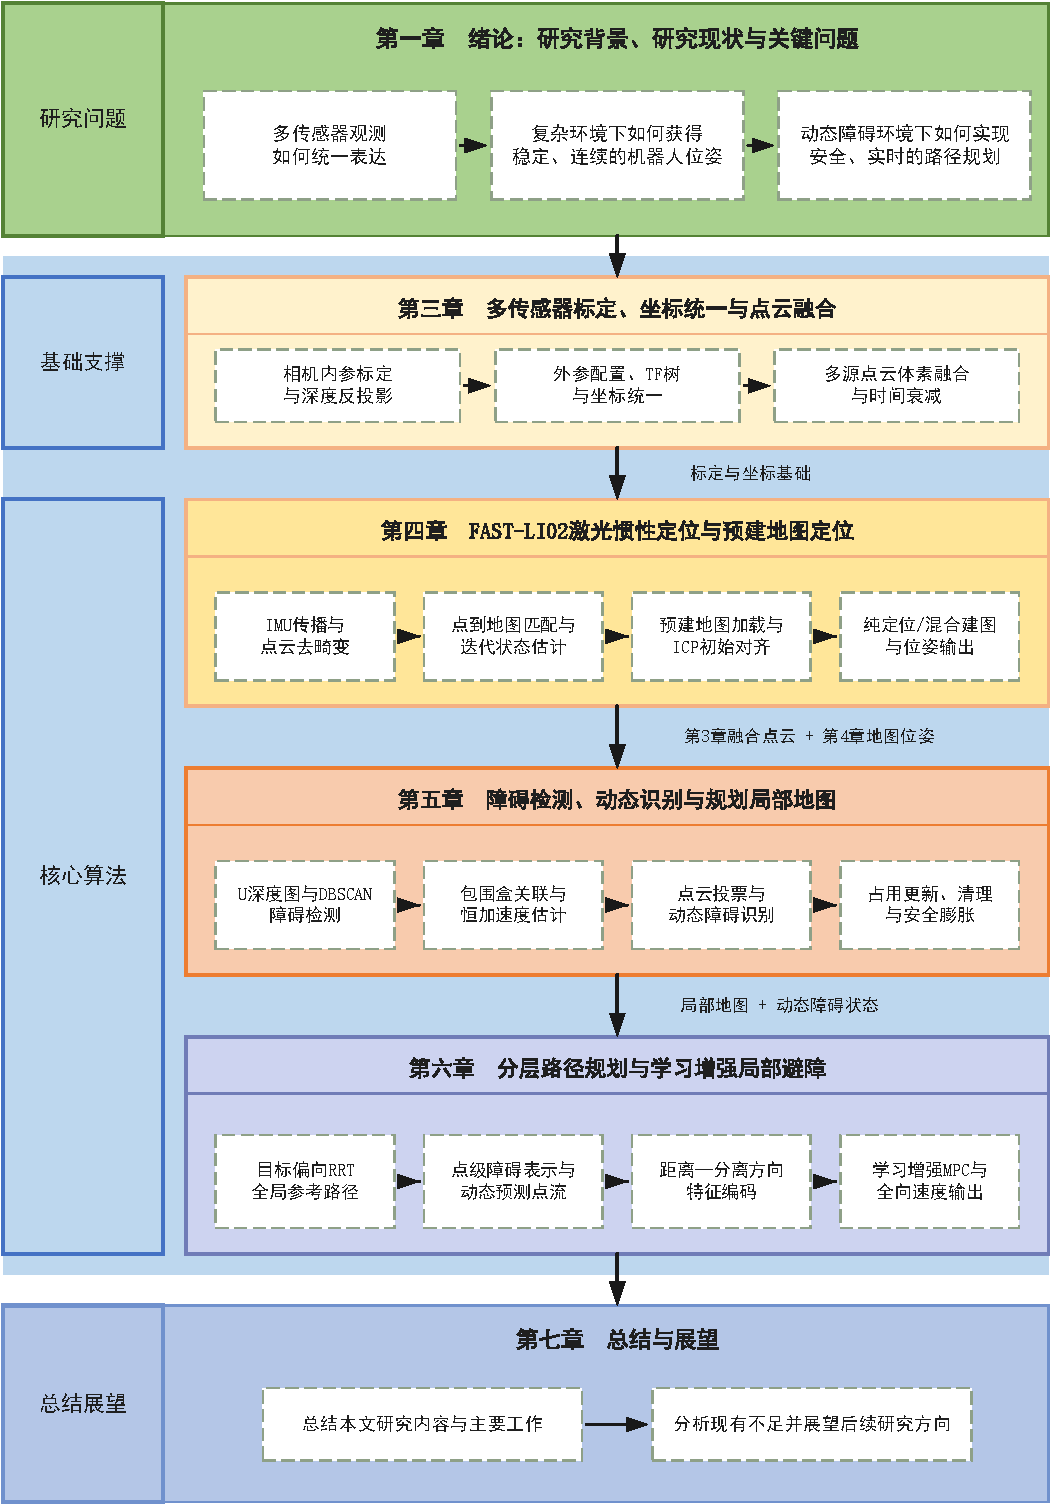
\includegraphics[width=\textwidth]{pic/论文框架图.pdf}
    \caption{本文研究内容与技术路线框架}
    \label{fig:论文框架图}
\end{figure}

围绕变电站运维搬运机器人在复杂、受限和动态环境中的自主导航需求，本文重点研究多传感器数据处理、激光惯性定位、障碍物检测与跟踪以及分层路径规划等关键问题，具体研究内容如下。

第三章阐述了多传感器标定与坐标变换方法。首先，定义了世界坐标系、机器人基坐标系、激光雷达坐标系和相机坐标系，并建立了各坐标系之间的齐次变换关系；其次，针对双目深度相机介绍了针孔成像模型、镜头畸变模型和张正友标定法，并完成了Gemini335L深度相机红外图像流的内参标定；然后，结合传感器的机械安装关系配置激光雷达、深度相机与机器人基坐标系之间的静态外参及TF变换；最后，研究了深度图像反投影、点云坐标变换以及多传感器点云融合方法，采用局部体素地图对激光雷达和深度相机观测进行统一表达，并通过差异化融合和时间衰减机制为后续障碍物检测与路径规划提供稳定的局部环境观测。

第四章研究了基于FAST\_LIO2的激光里程计定位方法。首先分析了激光雷达与惯性测量单元紧耦合定位的基本原理，介绍了IMU状态传播、点云去畸变、直接点到地图匹配、迭代误差状态卡尔曼滤波以及基于ikd-Tree的增量地图维护方法；在此基础上，面向变电站等具有预建地图的应用场景，设计了预建点云地图加载、地图降采样、初始位姿估计和ICP精配准相结合的定位初始化流程；进一步研究了固定预建地图下的纯定位模式和允许在线更新的混合建图模式，明确了定位系统向上层感知和规划模块输出全局位姿、连续轨迹及当前帧点云的接口，为机器人在复杂环境中的稳定定位提供基础。

第五章研究了运维机器人障碍检测与环境感知方法。针对小型移动机器人计算资源有限、深度相机视场受限以及复杂环境中单一传感器容易误检的问题，构建了基于深度图像和点云数据融合的轻量级障碍物检测与跟踪框架。首先介绍了K-Means和DBSCAN点云聚类方法，并分别利用U深度图检测器和DBSCAN检测器提取障碍物信息；随后对不同检测器的结果进行关联与融合，结合包围盒运动状态、点云运动一致性和点云投票机制识别动态障碍物，并利用滤波方法估计障碍物的速度和加速度状态；最后，基于第3章输出的多传感器融合观测以及本章获得的障碍物检测与跟踪结果，研究障碍物检测后的局部地图更新、自由空间确认、陈旧占用清理和障碍物膨胀方法，构建面向路径规划安全约束的局部环境表示。

第六章研究了分层路径规划与学习增强局部避障方法。针对变电站环境中设备密集、通道狭窄、障碍物形状复杂以及动态障碍物持续变化等问题，构建了“全局参考引导—局部滚动优化—底盘速度执行”的分层规划框架。全局规划层采用目标偏向RRT生成二维拓扑可行的参考路径，并通过直连检查、线段碰撞检测、超时处理、路径裁剪、路径平滑及平滑后碰撞复检提高全局路径的工程可用性；局部规划层建立全向移动底盘运动模型，将第5章输出的障碍物边界点和动态状态估计结果转换为点级障碍表示及预测点流，并引入点级几何编码器学习障碍边界与机器人轮廓之间的距离和分离方向特征，在此基础上构建带误差补偿、控制约束和松弛变量的学习增强MPC；最后，设计了优化失败、求解超时、碰撞风险和目标到达等异常状态处理机制，将MPC输出的首个最优控制量直接映射为全向底盘的速度指令，并通过仿真与实物实验对规划方法的可行性和实时性进行验证。

综上，本文围绕机器人导航系统中的“传感器数据统一—机器人状态估计—环境障碍理解—路径规划与控制执行”这一技术链条展开研究，形成了从多源感知输入到全向底盘速度输出的导航算法体系。